\documentclass[1p]{elsarticle_modified}
%\bibliographystyle{elsarticle-num}

%\usepackage[colorlinks]{hyperref}
%\usepackage{abbrmath_seonhwa} %\Abb, \Ascr, \Acal ,\Abf, \Afrak
\usepackage{amsfonts}
\usepackage{amssymb}
\usepackage{amsmath}
\usepackage{amsthm}
\usepackage{scalefnt}
\usepackage{amsbsy}
\usepackage{kotex}
\usepackage{caption}
\usepackage{subfig}
\usepackage{color}
\usepackage{graphicx}
\usepackage{xcolor} %% white, black, red, green, blue, cyan, magenta, yellow
\usepackage{float}
\usepackage{setspace}
\usepackage{hyperref}

\usepackage{tikz}
\usetikzlibrary{arrows}

\usepackage{multirow}
\usepackage{array} % fixed length table
\usepackage{hhline}

%%%%%%%%%%%%%%%%%%%%%
\makeatletter
\renewcommand*\env@matrix[1][\arraystretch]{%
	\edef\arraystretch{#1}%
	\hskip -\arraycolsep
	\let\@ifnextchar\new@ifnextchar
	\array{*\c@MaxMatrixCols c}}
\makeatother %https://tex.stackexchange.com/questions/14071/how-can-i-increase-the-line-spacing-in-a-matrix
%%%%%%%%%%%%%%%

\usepackage[normalem]{ulem}

\newcommand{\msout}[1]{\ifmmode\text{\sout{\ensuremath{#1}}}\else\sout{#1}\fi}
%SOURCE: \msout is \stkout macro in https://tex.stackexchange.com/questions/20609/strikeout-in-math-mode

\newcommand{\cancel}[1]{
	\ifmmode
	{\color{red}\msout{#1}}
	\else
	{\color{red}\sout{#1}}
	\fi
}

\newcommand{\add}[1]{
	{\color{blue}\uwave{#1}}
}

\newcommand{\replace}[2]{
	\ifmmode
	{\color{red}\msout{#1}}{\color{blue}\uwave{#2}}
	\else
	{\color{red}\sout{#1}}{\color{blue}\uwave{#2}}
	\fi
}

\newcommand{\Sol}{\mathcal{S}} %segment
\newcommand{\D}{D} %diagram
\newcommand{\A}{\mathcal{A}} %arc


%%%%%%%%%%%%%%%%%%%%%%%%%%%%%5 test

\def\sl{\operatorname{\textup{SL}}(2,\Cbb)}
\def\psl{\operatorname{\textup{PSL}}(2,\Cbb)}
\def\quan{\mkern 1mu \triangleright \mkern 1mu}

\theoremstyle{definition}
\newtheorem{thm}{Theorem}[section]
\newtheorem{prop}[thm]{Proposition}
\newtheorem{lem}[thm]{Lemma}
\newtheorem{ques}[thm]{Question}
\newtheorem{cor}[thm]{Corollary}
\newtheorem{defn}[thm]{Definition}
\newtheorem{exam}[thm]{Example}
\newtheorem{rmk}[thm]{Remark}
\newtheorem{alg}[thm]{Algorithm}

\newcommand{\I}{\sqrt{-1}}
\begin{document}

%\begin{frontmatter}
%
%\title{Boundary parabolic representations of knots up to 8 crossings}
%
%%% Group authors per affiliation:
%\author{Yunhi Cho} 
%\address{Department of Mathematics, University of Seoul, Seoul, Korea}
%\ead{yhcho@uos.ac.kr}
%
%
%\author{Seonhwa Kim} %\fnref{s_kim}}
%\address{Center for Geometry and Physics, Institute for Basic Science, Pohang, 37673, Korea}
%\ead{ryeona17@ibs.re.kr}
%
%\author{Hyuk Kim}
%\address{Department of Mathematical Sciences, Seoul National University, Seoul 08826, Korea}
%\ead{hyukkim@snu.ac.kr}
%
%\author{Seokbeom Yoon}
%\address{Department of Mathematical Sciences, Seoul National University, Seoul, 08826,  Korea}
%\ead{sbyoon15@snu.ac.kr}
%
%\begin{abstract}
%We find all boundary parabolic representation of knots up to 8 crossings.
%
%\end{abstract}
%\begin{keyword}
%    \MSC[2010] 57M25 
%\end{keyword}
%
%\end{frontmatter}

%\linenumbers
%\tableofcontents
%
\newcommand\colored[1]{\textcolor{white}{\rule[-0.35ex]{0.8em}{1.4ex}}\kern-0.8em\color{red} #1}%
%\newcommand\colored[1]{\textcolor{white}{ #1}\kern-2.17ex	\textcolor{white}{ #1}\kern-1.81ex	\textcolor{white}{ #1}\kern-2.15ex\color{red}#1	}

{\Large $\underline{12n_{0455}~(K12n_{0455})}$}

\setlength{\tabcolsep}{10pt}
\renewcommand{\arraystretch}{1.6}
\vspace{1cm}\begin{tabular}{m{100pt}>{\centering\arraybackslash}m{274pt}}
\multirow{5}{120pt}{
	\centering
	\includegraphics[width=112pt]{../../../GIT/diagram.site/Diagrams/png/2544_12n_0455.png}\\
\ \ \ A knot diagram\footnotemark}&
\allowdisplaybreaks
\textbf{Linearized knot diagam} \\
\cline{2-2}
 &
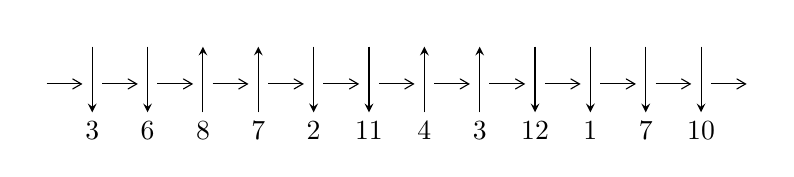
\begin{tikzpicture}[x=20pt, y=17pt]
	% nodes
	\node (C0) at (0, 0) {};
	\node (C1) at (1, 0) {};
	\node (C1U) at (1, +1) {};
	\node (C1D) at (1, -1) {3};

	\node (C2) at (2, 0) {};
	\node (C2U) at (2, +1) {};
	\node (C2D) at (2, -1) {6};

	\node (C3) at (3, 0) {};
	\node (C3U) at (3, +1) {};
	\node (C3D) at (3, -1) {8};

	\node (C4) at (4, 0) {};
	\node (C4U) at (4, +1) {};
	\node (C4D) at (4, -1) {7};

	\node (C5) at (5, 0) {};
	\node (C5U) at (5, +1) {};
	\node (C5D) at (5, -1) {2};

	\node (C6) at (6, 0) {};
	\node (C6U) at (6, +1) {};
	\node (C6D) at (6, -1) {11};

	\node (C7) at (7, 0) {};
	\node (C7U) at (7, +1) {};
	\node (C7D) at (7, -1) {4};

	\node (C8) at (8, 0) {};
	\node (C8U) at (8, +1) {};
	\node (C8D) at (8, -1) {3};

	\node (C9) at (9, 0) {};
	\node (C9U) at (9, +1) {};
	\node (C9D) at (9, -1) {12};

	\node (C10) at (10, 0) {};
	\node (C10U) at (10, +1) {};
	\node (C10D) at (10, -1) {1};

	\node (C11) at (11, 0) {};
	\node (C11U) at (11, +1) {};
	\node (C11D) at (11, -1) {7};

	\node (C12) at (12, 0) {};
	\node (C12U) at (12, +1) {};
	\node (C12D) at (12, -1) {10};
	\node (C13) at (13, 0) {};

	% arrows
	\draw[->,>={angle 60}]
	(C0) edge (C1) (C1) edge (C2) (C2) edge (C3) (C3) edge (C4) (C4) edge (C5) (C5) edge (C6) (C6) edge (C7) (C7) edge (C8) (C8) edge (C9) (C9) edge (C10) (C10) edge (C11) (C11) edge (C12) (C12) edge (C13) ;	\draw[->,>=stealth]
	(C1U) edge (C1D) (C2U) edge (C2D) (C3D) edge (C3U) (C4D) edge (C4U) (C5U) edge (C5D) (C6U) edge (C6D) (C7D) edge (C7U) (C8D) edge (C8U) (C9U) edge (C9D) (C10U) edge (C10D) (C11U) edge (C11D) (C12U) edge (C12D) ;
	\end{tikzpicture} \\
\hhline{~~} \\& 
\textbf{Solving Sequence} \\ \cline{2-2} 
 &
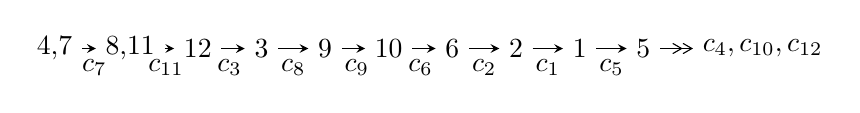
\begin{tikzpicture}[x=23pt, y=7pt]
	% node
	\node (A0) at (-1/8, 0) {4,7};
	\node (A1) at (17/16, 0) {8,11};
	\node (A2) at (17/8, 0) {12};
	\node (A3) at (25/8, 0) {3};
	\node (A4) at (33/8, 0) {9};
	\node (A5) at (41/8, 0) {10};
	\node (A6) at (49/8, 0) {6};
	\node (A7) at (57/8, 0) {2};
	\node (A8) at (65/8, 0) {1};
	\node (A9) at (73/8, 0) {5};
	\node (C1) at (1/2, -1) {$c_{7}$};
	\node (C2) at (13/8, -1) {$c_{11}$};
	\node (C3) at (21/8, -1) {$c_{3}$};
	\node (C4) at (29/8, -1) {$c_{8}$};
	\node (C5) at (37/8, -1) {$c_{9}$};
	\node (C6) at (45/8, -1) {$c_{6}$};
	\node (C7) at (53/8, -1) {$c_{2}$};
	\node (C8) at (61/8, -1) {$c_{1}$};
	\node (C9) at (69/8, -1) {$c_{5}$};
	\node (A10) at (11, 0) {$c_{4},c_{10},c_{12}$};

	% edge
	\draw[->,>=stealth]	
	(A0) edge (A1) (A1) edge (A2) (A2) edge (A3) (A3) edge (A4) (A4) edge (A5) (A5) edge (A6) (A6) edge (A7) (A7) edge (A8) (A8) edge (A9) ;
	\draw[->>,>={angle 60}]	
	(A9) edge (A10);
\end{tikzpicture} \\ 

\end{tabular} \\

\footnotetext{
The image of knot diagram is generated by the software ``\textbf{Draw programme}" developed by Andrew Bartholomew(\url{http://www.layer8.co.uk/maths/draw/index.htm\#Running-draw}), where we modified some parts for our purpose(\url{https://github.com/CATsTAILs/LinksPainter}).
}\phantom \\ \newline 
\centering \textbf{Ideals for irreducible components\footnotemark of $X_{\text{par}}$} 
 
\begin{align*}
I^u_{1}&=\langle 
3.50811\times10^{48} u^{55}+5.98520\times10^{48} u^{54}+\cdots+2.69358\times10^{47} b+4.89292\times10^{49},\\
\phantom{I^u_{1}}&\phantom{= \langle  }2.55712\times10^{50} u^{55}+4.32535\times10^{50} u^{54}+\cdots+5.65653\times10^{48} a+3.41422\times10^{51},\;u^{56}+2 u^{55}+\cdots+44 u+4\rangle \\
I^u_{2}&=\langle 
b,\;3 a+u+1,\;u^2- u+1\rangle \\
I^u_{3}&=\langle 
- a u+9 b-4 a+u-5,\;2 a^2- a u+5 u-9,\;u^2+2\rangle \\
\\
I^v_{1}&=\langle 
a,\;b+v+2,\;v^2+3 v+1\rangle \\
\end{align*}
\raggedright * 4 irreducible components of $\dim_{\mathbb{C}}=0$, with total 64 representations.\\
\footnotetext{All coefficients of polynomials are rational numbers. But the coefficients are sometimes approximated in decimal forms when there is not enough margin.}
\newpage
\renewcommand{\arraystretch}{1}
\centering \section*{I. $I^u_{1}= \langle 3.51\times10^{48} u^{55}+5.99\times10^{48} u^{54}+\cdots+2.69\times10^{47} b+4.89\times10^{49},\;2.56\times10^{50} u^{55}+4.33\times10^{50} u^{54}+\cdots+5.66\times10^{48} a+3.41\times10^{51},\;u^{56}+2 u^{55}+\cdots+44 u+4 \rangle$}
\flushleft \textbf{(i) Arc colorings}\\
\begin{tabular}{m{7pt} m{180pt} m{7pt} m{180pt} }
\flushright $a_{4}=$&$\begin{pmatrix}0\\u\end{pmatrix}$ \\
\flushright $a_{7}=$&$\begin{pmatrix}1\\0\end{pmatrix}$ \\
\flushright $a_{8}=$&$\begin{pmatrix}1\\- u^2\end{pmatrix}$ \\
\flushright $a_{11}=$&$\begin{pmatrix}-45.2065 u^{55}-76.4665 u^{54}+\cdots-4615.91 u-603.589\\-13.0239 u^{55}-22.2202 u^{54}+\cdots-1365.32 u-181.651\end{pmatrix}$ \\
\flushright $a_{12}=$&$\begin{pmatrix}-32.1825 u^{55}-54.2463 u^{54}+\cdots-3250.59 u-421.938\\-13.0239 u^{55}-22.2202 u^{54}+\cdots-1365.32 u-181.651\end{pmatrix}$ \\
\flushright $a_{3}=$&$\begin{pmatrix}- u\\u^3+u\end{pmatrix}$ \\
\flushright $a_{9}=$&$\begin{pmatrix}u^2+1\\- u^4-2 u^2\end{pmatrix}$ \\
\flushright $a_{10}=$&$\begin{pmatrix}33.0942 u^{55}+56.4532 u^{54}+\cdots+3417.51 u+449.013\\-28.0321 u^{55}-47.5425 u^{54}+\cdots-2839.05 u-370.800\end{pmatrix}$ \\
\flushright $a_{6}=$&$\begin{pmatrix}27.7411 u^{55}+46.8651 u^{54}+\cdots+2813.09 u+362.109\\24.2434 u^{55}+41.0750 u^{54}+\cdots+2515.79 u+329.906\end{pmatrix}$ \\
\flushright $a_{2}=$&$\begin{pmatrix}-27.7411 u^{55}-46.8651 u^{54}+\cdots-2813.09 u-362.109\\27.3678 u^{55}+46.3317 u^{54}+\cdots+2783.98 u+364.375\end{pmatrix}$ \\
\flushright $a_{1}=$&$\begin{pmatrix}-28.1461 u^{55}-47.2742 u^{54}+\cdots-2852.14 u-366.930\\28.0321 u^{55}+47.5425 u^{54}+\cdots+2839.05 u+370.800\end{pmatrix}$ \\
\flushright $a_{5}=$&$\begin{pmatrix}u\\u\end{pmatrix}$\\&\end{tabular}
\flushleft \textbf{(ii) Obstruction class $= -1$}\\~\\
\flushleft \textbf{(iii) Cusp Shapes $= -46.3572 u^{55}-80.1696 u^{54}+\cdots-5049.53 u-698.513$}\\~\\
\newpage\renewcommand{\arraystretch}{1}
\flushleft \textbf{(iv) u-Polynomials at the component}\newline \\
\begin{tabular}{m{50pt}|m{274pt}}
Crossings & \hspace{64pt}u-Polynomials at each crossing \\
\hline $$\begin{aligned}c_{1}\end{aligned}$$&$\begin{aligned}
&u^{56}+24 u^{55}+\cdots+25165 u+361
\end{aligned}$\\
\hline $$\begin{aligned}c_{2},c_{5}\end{aligned}$$&$\begin{aligned}
&u^{56}+4 u^{55}+\cdots-41 u+19
\end{aligned}$\\
\hline $$\begin{aligned}c_{3},c_{4},c_{7}\\c_{8}\end{aligned}$$&$\begin{aligned}
&u^{56}+2 u^{55}+\cdots+44 u+4
\end{aligned}$\\
\hline $$\begin{aligned}c_{6},c_{11}\end{aligned}$$&$\begin{aligned}
&u^{56}-2 u^{55}+\cdots-108 u+36
\end{aligned}$\\
\hline $$\begin{aligned}c_{9},c_{10},c_{12}\end{aligned}$$&$\begin{aligned}
&u^{56}-6 u^{55}+\cdots+31 u+9
\end{aligned}$\\
\hline
\end{tabular}\\~\\
\newpage\renewcommand{\arraystretch}{1}
\flushleft \textbf{(v) Riley Polynomials at the component}\newline \\
\begin{tabular}{m{50pt}|m{274pt}}
Crossings & \hspace{64pt}Riley Polynomials at each crossing \\
\hline $$\begin{aligned}c_{1}\end{aligned}$$&$\begin{aligned}
&y^{56}+16 y^{55}+\cdots-427912989 y+130321
\end{aligned}$\\
\hline $$\begin{aligned}c_{2},c_{5}\end{aligned}$$&$\begin{aligned}
&y^{56}-24 y^{55}+\cdots-25165 y+361
\end{aligned}$\\
\hline $$\begin{aligned}c_{3},c_{4},c_{7}\\c_{8}\end{aligned}$$&$\begin{aligned}
&y^{56}+50 y^{55}+\cdots-464 y+16
\end{aligned}$\\
\hline $$\begin{aligned}c_{6},c_{11}\end{aligned}$$&$\begin{aligned}
&y^{56}-24 y^{55}+\cdots-17784 y+1296
\end{aligned}$\\
\hline $$\begin{aligned}c_{9},c_{10},c_{12}\end{aligned}$$&$\begin{aligned}
&y^{56}-50 y^{55}+\cdots+605 y+81
\end{aligned}$\\
\hline
\end{tabular}\\~\\
\newpage\flushleft \textbf{(vi) Complex Volumes and Cusp Shapes}
$$\begin{array}{c|c|c}  
\text{Solutions to }I^u_{1}& \I (\text{vol} + \sqrt{-1}CS) & \text{Cusp shape}\\
 \hline 
\begin{aligned}
u &= -0.357425 + 0.939932 I \\
a &= -0.508559 + 0.668079 I \\
b &= -0.709734 + 0.751032 I\end{aligned}
 & \phantom{-}0.10978 + 1.51144 I & \phantom{-0.000000 } 0 \\ \hline\begin{aligned}
u &= -0.357425 - 0.939932 I \\
a &= -0.508559 - 0.668079 I \\
b &= -0.709734 - 0.751032 I\end{aligned}
 & \phantom{-}0.10978 - 1.51144 I & \phantom{-0.000000 } 0 \\ \hline\begin{aligned}
u &= \phantom{-}0.916252 + 0.279624 I \\
a &= -0.263707 - 0.445797 I \\
b &= -0.801946 + 0.644092 I\end{aligned}
 & \phantom{-}0.01268 + 4.06286 I & -6.20066 - 5.47620 I \\ \hline\begin{aligned}
u &= \phantom{-}0.916252 - 0.279624 I \\
a &= -0.263707 + 0.445797 I \\
b &= -0.801946 - 0.644092 I\end{aligned}
 & \phantom{-}0.01268 - 4.06286 I & -6.20066 + 5.47620 I \\ \hline\begin{aligned}
u &= -0.870458 + 0.356425 I \\
a &= -0.654647 + 0.719979 I \\
b &= -1.104950 - 0.815677 I\end{aligned}
 & -2.43509 - 10.45620 I & -7.88871 + 7.69025 I \\ \hline\begin{aligned}
u &= -0.870458 - 0.356425 I \\
a &= -0.654647 - 0.719979 I \\
b &= -1.104950 + 0.815677 I\end{aligned}
 & -2.43509 + 10.45620 I & -7.88871 - 7.69025 I \\ \hline\begin{aligned}
u &= -0.672518 + 0.823461 I \\
a &= \phantom{-}0.189263 - 0.600931 I \\
b &= \phantom{-}0.930657 - 0.635738 I\end{aligned}
 & -3.85927 + 5.20665 I & \phantom{-0.000000 } 0 \\ \hline\begin{aligned}
u &= -0.672518 - 0.823461 I \\
a &= \phantom{-}0.189263 + 0.600931 I \\
b &= \phantom{-}0.930657 + 0.635738 I\end{aligned}
 & -3.85927 - 5.20665 I & \phantom{-0.000000 } 0 \\ \hline\begin{aligned}
u &= \phantom{-}0.138429 + 1.163150 I \\
a &= \phantom{-}2.11508 + 0.18189 I \\
b &= \phantom{-}0.981368 - 0.595861 I\end{aligned}
 & -3.70144 - 0.59074 I & \phantom{-0.000000 } 0 \\ \hline\begin{aligned}
u &= \phantom{-}0.138429 - 1.163150 I \\
a &= \phantom{-}2.11508 - 0.18189 I \\
b &= \phantom{-}0.981368 + 0.595861 I\end{aligned}
 & -3.70144 + 0.59074 I & \phantom{-0.000000 } 0\\
 \hline 
 \end{array}$$\newpage$$\begin{array}{c|c|c}  
\text{Solutions to }I^u_{1}& \I (\text{vol} + \sqrt{-1}CS) & \text{Cusp shape}\\
 \hline 
\begin{aligned}
u &= -0.796673 + 0.217361 I \\
a &= \phantom{-}0.732692 - 0.735103 I \\
b &= \phantom{-}1.047550 + 0.754047 I\end{aligned}
 & \phantom{-}2.36888 - 5.77663 I & -3.49704 + 6.12922 I \\ \hline\begin{aligned}
u &= -0.796673 - 0.217361 I \\
a &= \phantom{-}0.732692 + 0.735103 I \\
b &= \phantom{-}1.047550 - 0.754047 I\end{aligned}
 & \phantom{-}2.36888 + 5.77663 I & -3.49704 - 6.12922 I \\ \hline\begin{aligned}
u &= -0.813175\phantom{ +0.000000I} \\
a &= \phantom{-}0.696477\phantom{ +0.000000I} \\
b &= -0.998455\phantom{ +0.000000I}\end{aligned}
 & -7.46368\phantom{ +0.000000I} & -11.8850\phantom{ +0.000000I} \\ \hline\begin{aligned}
u &= \phantom{-}0.786622 + 0.053183 I \\
a &= \phantom{-}0.235360 + 0.517834 I \\
b &= \phantom{-}0.691285 - 0.845614 I\end{aligned}
 & \phantom{-}3.46294 + 0.21119 I &                  -6
-0.626193 + 0. 10   I\phantom{ +0.000000I} \\ \hline\begin{aligned}
u &= \phantom{-}0.786622 - 0.053183 I \\
a &= \phantom{-}0.235360 - 0.517834 I \\
b &= \phantom{-}0.691285 + 0.845614 I\end{aligned}
 & \phantom{-}3.46294 - 0.21119 I &                  -6
-0.626193 + 0. 10   I\phantom{ +0.000000I} \\ \hline\begin{aligned}
u &= \phantom{-}0.686659 + 1.019540 I \\
a &= \phantom{-}0.152248 + 0.372794 I \\
b &= \phantom{-}0.649441 + 0.261695 I\end{aligned}
 & -2.10341 + 1.46035 I & \phantom{-0.000000 } 0 \\ \hline\begin{aligned}
u &= \phantom{-}0.686659 - 1.019540 I \\
a &= \phantom{-}0.152248 - 0.372794 I \\
b &= \phantom{-}0.649441 - 0.261695 I\end{aligned}
 & -2.10341 - 1.46035 I & \phantom{-0.000000 } 0 \\ \hline\begin{aligned}
u &= \phantom{-}0.363201 + 1.199600 I \\
a &= \phantom{-}0.050246 - 0.686716 I \\
b &= -0.360705 - 0.909449 I\end{aligned}
 & -0.05819 + 3.93594 I & \phantom{-0.000000 } 0 \\ \hline\begin{aligned}
u &= \phantom{-}0.363201 - 1.199600 I \\
a &= \phantom{-}0.050246 + 0.686716 I \\
b &= -0.360705 + 0.909449 I\end{aligned}
 & -0.05819 - 3.93594 I & \phantom{-0.000000 } 0 \\ \hline\begin{aligned}
u &= \phantom{-}0.694825 + 0.177977 I \\
a &= -0.175933 + 0.543419 I \\
b &= -0.679667 - 1.057170 I\end{aligned}
 & -1.07651 + 3.71517 I & -5.64023 - 4.49934 I\\
 \hline 
 \end{array}$$\newpage$$\begin{array}{c|c|c}  
\text{Solutions to }I^u_{1}& \I (\text{vol} + \sqrt{-1}CS) & \text{Cusp shape}\\
 \hline 
\begin{aligned}
u &= \phantom{-}0.694825 - 0.177977 I \\
a &= -0.175933 - 0.543419 I \\
b &= -0.679667 + 1.057170 I\end{aligned}
 & -1.07651 - 3.71517 I & -5.64023 + 4.49934 I \\ \hline\begin{aligned}
u &= -0.222724 + 1.263850 I \\
a &= \phantom{-}0.746580 - 0.478205 I \\
b &= \phantom{-}0.691653 - 0.998010 I\end{aligned}
 & -4.19144 - 2.28903 I & \phantom{-0.000000 } 0 \\ \hline\begin{aligned}
u &= -0.222724 - 1.263850 I \\
a &= \phantom{-}0.746580 + 0.478205 I \\
b &= \phantom{-}0.691653 + 0.998010 I\end{aligned}
 & -4.19144 + 2.28903 I & \phantom{-0.000000 } 0 \\ \hline\begin{aligned}
u &= \phantom{-}0.212493 + 0.663538 I \\
a &= -0.798139 + 0.138816 I \\
b &= -0.332186 + 0.507658 I\end{aligned}
 & -0.238433 + 1.252040 I & -2.82125 - 5.02862 I \\ \hline\begin{aligned}
u &= \phantom{-}0.212493 - 0.663538 I \\
a &= -0.798139 - 0.138816 I \\
b &= -0.332186 - 0.507658 I\end{aligned}
 & -0.238433 - 1.252040 I & -2.82125 + 5.02862 I \\ \hline\begin{aligned}
u &= -0.125478 + 1.304740 I \\
a &= -0.84758 + 1.18038 I \\
b &= -0.758335 - 0.376703 I\end{aligned}
 & -6.56363 - 1.59389 I & \phantom{-0.000000 } 0 \\ \hline\begin{aligned}
u &= -0.125478 - 1.304740 I \\
a &= -0.84758 - 1.18038 I \\
b &= -0.758335 + 0.376703 I\end{aligned}
 & -6.56363 + 1.59389 I & \phantom{-0.000000 } 0 \\ \hline\begin{aligned}
u &= -0.098940 + 1.329620 I \\
a &= -2.59434 + 0.37087 I \\
b &= -1.79675 + 0.14155 I\end{aligned}
 & -14.6366 - 1.4158 I & \phantom{-0.000000 } 0 \\ \hline\begin{aligned}
u &= -0.098940 - 1.329620 I \\
a &= -2.59434 - 0.37087 I \\
b &= -1.79675 - 0.14155 I\end{aligned}
 & -14.6366 + 1.4158 I & \phantom{-0.000000 } 0 \\ \hline\begin{aligned}
u &= \phantom{-}0.326495 + 1.296350 I \\
a &= -1.68324 - 0.31227 I \\
b &= -0.993147 + 0.745876 I\end{aligned}
 & -0.74471 + 4.21273 I & \phantom{-0.000000 } 0\\
 \hline 
 \end{array}$$\newpage$$\begin{array}{c|c|c}  
\text{Solutions to }I^u_{1}& \I (\text{vol} + \sqrt{-1}CS) & \text{Cusp shape}\\
 \hline 
\begin{aligned}
u &= \phantom{-}0.326495 - 1.296350 I \\
a &= -1.68324 + 0.31227 I \\
b &= -0.993147 - 0.745876 I\end{aligned}
 & -0.74471 - 4.21273 I & \phantom{-0.000000 } 0 \\ \hline\begin{aligned}
u &= -0.261932 + 1.315040 I \\
a &= \phantom{-}2.39778 - 0.42809 I \\
b &= \phantom{-}1.291360 + 0.390540 I\end{aligned}
 & -4.85102 - 4.10127 I & \phantom{-0.000000 } 0 \\ \hline\begin{aligned}
u &= -0.261932 - 1.315040 I \\
a &= \phantom{-}2.39778 + 0.42809 I \\
b &= \phantom{-}1.291360 - 0.390540 I\end{aligned}
 & -4.85102 + 4.10127 I & \phantom{-0.000000 } 0 \\ \hline\begin{aligned}
u &= -0.646445 + 0.063362 I \\
a &= -0.928542 + 0.691777 I \\
b &= -0.988563 - 0.589361 I\end{aligned}
 & -0.514192 - 0.792549 I & -4.90653 + 2.84844 I \\ \hline\begin{aligned}
u &= -0.646445 - 0.063362 I \\
a &= -0.928542 - 0.691777 I \\
b &= -0.988563 + 0.589361 I\end{aligned}
 & -0.514192 + 0.792549 I & -4.90653 - 2.84844 I \\ \hline\begin{aligned}
u &= -0.341280 + 1.316540 I \\
a &= \phantom{-}0.817304 - 0.783388 I \\
b &= \phantom{-}1.073100 + 0.391226 I\end{aligned}
 & -11.62750 - 4.16517 I & \phantom{-0.000000 } 0 \\ \hline\begin{aligned}
u &= -0.341280 - 1.316540 I \\
a &= \phantom{-}0.817304 + 0.783388 I \\
b &= \phantom{-}1.073100 - 0.391226 I\end{aligned}
 & -11.62750 + 4.16517 I & \phantom{-0.000000 } 0 \\ \hline\begin{aligned}
u &= \phantom{-}0.288431 + 1.366350 I \\
a &= \phantom{-}0.141585 + 0.969892 I \\
b &= \phantom{-}0.55694 + 1.31146 I\end{aligned}
 & -5.96654 + 7.30226 I & \phantom{-0.000000 } 0 \\ \hline\begin{aligned}
u &= \phantom{-}0.288431 - 1.366350 I \\
a &= \phantom{-}0.141585 - 0.969892 I \\
b &= \phantom{-}0.55694 - 1.31146 I\end{aligned}
 & -5.96654 - 7.30226 I & \phantom{-0.000000 } 0 \\ \hline\begin{aligned}
u &= \phantom{-}0.085846 + 1.404690 I \\
a &= -0.72751 - 1.48763 I \\
b &= \phantom{-}0.118836 + 0.664953 I\end{aligned}
 & -8.80079 + 0.29511 I & \phantom{-0.000000 } 0\\
 \hline 
 \end{array}$$\newpage$$\begin{array}{c|c|c}  
\text{Solutions to }I^u_{1}& \I (\text{vol} + \sqrt{-1}CS) & \text{Cusp shape}\\
 \hline 
\begin{aligned}
u &= \phantom{-}0.085846 - 1.404690 I \\
a &= -0.72751 + 1.48763 I \\
b &= \phantom{-}0.118836 - 0.664953 I\end{aligned}
 & -8.80079 - 0.29511 I & \phantom{-0.000000 } 0 \\ \hline\begin{aligned}
u &= -0.33202 + 1.39409 I \\
a &= -2.13548 + 0.45520 I \\
b &= -1.242450 - 0.672303 I\end{aligned}
 & -2.74251 - 9.86043 I & \phantom{-0.000000 } 0 \\ \hline\begin{aligned}
u &= -0.33202 - 1.39409 I \\
a &= -2.13548 - 0.45520 I \\
b &= -1.242450 + 0.672303 I\end{aligned}
 & -2.74251 + 9.86043 I & \phantom{-0.000000 } 0 \\ \hline\begin{aligned}
u &= -0.04599 + 1.47574 I \\
a &= \phantom{-}1.78492 - 0.56193 I \\
b &= \phantom{-}0.697621 - 0.210255 I\end{aligned}
 & -7.13747 + 0.98410 I & \phantom{-0.000000 } 0 \\ \hline\begin{aligned}
u &= -0.04599 - 1.47574 I \\
a &= \phantom{-}1.78492 + 0.56193 I \\
b &= \phantom{-}0.697621 + 0.210255 I\end{aligned}
 & -7.13747 - 0.98410 I & \phantom{-0.000000 } 0 \\ \hline\begin{aligned}
u &= \phantom{-}0.37725 + 1.42997 I \\
a &= \phantom{-}1.48324 + 0.27092 I \\
b &= \phantom{-}1.064050 - 0.776573 I\end{aligned}
 & -5.40146 + 8.69654 I & \phantom{-0.000000 } 0 \\ \hline\begin{aligned}
u &= \phantom{-}0.37725 - 1.42997 I \\
a &= \phantom{-}1.48324 - 0.27092 I \\
b &= \phantom{-}1.064050 + 0.776573 I\end{aligned}
 & -5.40146 - 8.69654 I & \phantom{-0.000000 } 0 \\ \hline\begin{aligned}
u &= -0.34531 + 1.47025 I \\
a &= \phantom{-}1.95103 - 0.36645 I \\
b &= \phantom{-}1.27086 + 0.84602 I\end{aligned}
 & -8.2789 - 14.8605 I & \phantom{-0.000000 } 0 \\ \hline\begin{aligned}
u &= -0.34531 - 1.47025 I \\
a &= \phantom{-}1.95103 + 0.36645 I \\
b &= \phantom{-}1.27086 - 0.84602 I\end{aligned}
 & -8.2789 + 14.8605 I & \phantom{-0.000000 } 0 \\ \hline\begin{aligned}
u &= \phantom{-}0.146752 + 0.464276 I \\
a &= \phantom{-}3.63219 + 0.90440 I \\
b &= \phantom{-}0.425085 - 0.514946 I\end{aligned}
 & -3.04021 - 0.77078 I & -13.4195 - 5.3259 I\\
 \hline 
 \end{array}$$\newpage$$\begin{array}{c|c|c}  
\text{Solutions to }I^u_{1}& \I (\text{vol} + \sqrt{-1}CS) & \text{Cusp shape}\\
 \hline 
\begin{aligned}
u &= \phantom{-}0.146752 - 0.464276 I \\
a &= \phantom{-}3.63219 - 0.90440 I \\
b &= \phantom{-}0.425085 + 0.514946 I\end{aligned}
 & -3.04021 + 0.77078 I & -13.4195 + 5.3259 I \\ \hline\begin{aligned}
u &= -0.07154 + 1.61009 I \\
a &= -1.293690 + 0.377349 I \\
b &= -1.078470 + 0.249906 I\end{aligned}
 & -12.46720 + 2.72041 I & \phantom{-0.000000 } 0 \\ \hline\begin{aligned}
u &= -0.07154 - 1.61009 I \\
a &= -1.293690 - 0.377349 I \\
b &= -1.078470 - 0.249906 I\end{aligned}
 & -12.46720 - 2.72041 I & \phantom{-0.000000 } 0 \\ \hline\begin{aligned}
u &= -0.308833\phantom{ +0.000000I} \\
a &= -4.42147\phantom{ +0.000000I} \\
b &= \phantom{-}0.567778\phantom{ +0.000000I}\end{aligned}
 & -2.38389\phantom{ +0.000000I} & \phantom{-}8.02900\phantom{ +0.000000I} \\ \hline\begin{aligned}
u &= -0.296374\phantom{ +0.000000I} \\
a &= \phantom{-}0.686807\phantom{ +0.000000I} \\
b &= \phantom{-}1.68419\phantom{ +0.000000I}\end{aligned}
 & -10.2992\phantom{ +0.000000I} & \phantom{-}9.48110\phantom{ +0.000000I} \\ \hline\begin{aligned}
u &= -0.250665\phantom{ +0.000000I} \\
a &= -2.26479\phantom{ +0.000000I} \\
b &= -0.539323\phantom{ +0.000000I}\end{aligned}
 & -1.17956\phantom{ +0.000000I} & -7.76820\phantom{ +0.000000I}\\
 \hline 
 \end{array}$$\newpage\newpage\renewcommand{\arraystretch}{1}
\centering \section*{II. $I^u_{2}= \langle b,\;3 a+u+1,\;u^2- u+1 \rangle$}
\flushleft \textbf{(i) Arc colorings}\\
\begin{tabular}{m{7pt} m{180pt} m{7pt} m{180pt} }
\flushright $a_{4}=$&$\begin{pmatrix}0\\u\end{pmatrix}$ \\
\flushright $a_{7}=$&$\begin{pmatrix}1\\0\end{pmatrix}$ \\
\flushright $a_{8}=$&$\begin{pmatrix}1\\- u+1\end{pmatrix}$ \\
\flushright $a_{11}=$&$\begin{pmatrix}-\frac{1}{3} u-\frac{1}{3}\\0\end{pmatrix}$ \\
\flushright $a_{12}=$&$\begin{pmatrix}-\frac{1}{3} u-\frac{1}{3}\\0\end{pmatrix}$ \\
\flushright $a_{3}=$&$\begin{pmatrix}- u\\u-1\end{pmatrix}$ \\
\flushright $a_{9}=$&$\begin{pmatrix}u\\- u+2\end{pmatrix}$ \\
\flushright $a_{10}=$&$\begin{pmatrix}\frac{2}{3} u-\frac{1}{3}\\- u+2\end{pmatrix}$ \\
\flushright $a_{6}=$&$\begin{pmatrix}1\\0\end{pmatrix}$ \\
\flushright $a_{2}=$&$\begin{pmatrix}-1\\u-1\end{pmatrix}$ \\
\flushright $a_{1}=$&$\begin{pmatrix}- u\\u-2\end{pmatrix}$ \\
\flushright $a_{5}=$&$\begin{pmatrix}u\\u\end{pmatrix}$\\&\end{tabular}
\flushleft \textbf{(ii) Obstruction class $= 1$}\\~\\
\flushleft \textbf{(iii) Cusp Shapes $= -\frac{20}{3} u-3$}\\~\\
\newpage\renewcommand{\arraystretch}{1}
\flushleft \textbf{(iv) u-Polynomials at the component}\newline \\
\begin{tabular}{m{50pt}|m{274pt}}
Crossings & \hspace{64pt}u-Polynomials at each crossing \\
\hline $$\begin{aligned}c_{1},c_{3},c_{4}\\c_{5}\end{aligned}$$&$\begin{aligned}
&u^2+u+1
\end{aligned}$\\
\hline $$\begin{aligned}c_{2},c_{7},c_{8}\end{aligned}$$&$\begin{aligned}
&u^2- u+1
\end{aligned}$\\
\hline $$\begin{aligned}c_{6},c_{11}\end{aligned}$$&$\begin{aligned}
&u^2
\end{aligned}$\\
\hline $$\begin{aligned}c_{9},c_{10}\end{aligned}$$&$\begin{aligned}
&(u-1)^2
\end{aligned}$\\
\hline $$\begin{aligned}c_{12}\end{aligned}$$&$\begin{aligned}
&(u+1)^2
\end{aligned}$\\
\hline
\end{tabular}\\~\\
\newpage\renewcommand{\arraystretch}{1}
\flushleft \textbf{(v) Riley Polynomials at the component}\newline \\
\begin{tabular}{m{50pt}|m{274pt}}
Crossings & \hspace{64pt}Riley Polynomials at each crossing \\
\hline $$\begin{aligned}c_{1},c_{2},c_{3}\\c_{4},c_{5},c_{7}\\c_{8}\end{aligned}$$&$\begin{aligned}
&y^2+y+1
\end{aligned}$\\
\hline $$\begin{aligned}c_{6},c_{11}\end{aligned}$$&$\begin{aligned}
&y^2
\end{aligned}$\\
\hline $$\begin{aligned}c_{9},c_{10},c_{12}\end{aligned}$$&$\begin{aligned}
&(y-1)^2
\end{aligned}$\\
\hline
\end{tabular}\\~\\
\newpage\flushleft \textbf{(vi) Complex Volumes and Cusp Shapes}
$$\begin{array}{c|c|c}  
\text{Solutions to }I^u_{2}& \I (\text{vol} + \sqrt{-1}CS) & \text{Cusp shape}\\
 \hline 
\begin{aligned}
u &= \phantom{-}0.500000 + 0.866025 I \\
a &= -0.500000 - 0.288675 I \\
b &= \phantom{-0.000000 } 0\end{aligned}
 & -1.64493 + 2.02988 I & -6.33333 - 5.77350 I \\ \hline\begin{aligned}
u &= \phantom{-}0.500000 - 0.866025 I \\
a &= -0.500000 + 0.288675 I \\
b &= \phantom{-0.000000 } 0\end{aligned}
 & -1.64493 - 2.02988 I & -6.33333 + 5.77350 I\\
 \hline 
 \end{array}$$\newpage\newpage\renewcommand{\arraystretch}{1}
\centering \section*{III. $I^u_{3}= \langle - a u+9 b-4 a+u-5,\;2 a^2- a u+5 u-9,\;u^2+2 \rangle$}
\flushleft \textbf{(i) Arc colorings}\\
\begin{tabular}{m{7pt} m{180pt} m{7pt} m{180pt} }
\flushright $a_{4}=$&$\begin{pmatrix}0\\u\end{pmatrix}$ \\
\flushright $a_{7}=$&$\begin{pmatrix}1\\0\end{pmatrix}$ \\
\flushright $a_{8}=$&$\begin{pmatrix}1\\2\end{pmatrix}$ \\
\flushright $a_{11}=$&$\begin{pmatrix}a\\\frac{1}{9} a u+\frac{4}{9} a-\frac{1}{9} u+\frac{5}{9}\end{pmatrix}$ \\
\flushright $a_{12}=$&$\begin{pmatrix}-\frac{1}{9} a u+\frac{5}{9} a+\frac{1}{9} u-\frac{5}{9}\\\frac{1}{9} a u+\frac{4}{9} a-\frac{1}{9} u+\frac{5}{9}\end{pmatrix}$ \\
\flushright $a_{3}=$&$\begin{pmatrix}- u\\- u\end{pmatrix}$ \\
\flushright $a_{9}=$&$\begin{pmatrix}-1\\0\end{pmatrix}$ \\
\flushright $a_{10}=$&$\begin{pmatrix}\frac{1}{2} u-2\\-\frac{1}{9} a u-\frac{4}{9} a+\frac{1}{9} u-\frac{14}{9}\end{pmatrix}$ \\
\flushright $a_{6}=$&$\begin{pmatrix}-\frac{1}{9} a u-\frac{4}{9} a+\frac{11}{18} u-\frac{14}{9}\\-\frac{1}{9} a u-\frac{4}{9} a+\frac{1}{9} u-\frac{14}{9}\end{pmatrix}$ \\
\flushright $a_{2}=$&$\begin{pmatrix}-\frac{1}{9} a u-\frac{4}{9} a-\frac{7}{18} u-\frac{14}{9}\\-\frac{1}{9} a u-\frac{4}{9} a-\frac{8}{9} u-\frac{14}{9}\end{pmatrix}$ \\
\flushright $a_{1}=$&$\begin{pmatrix}-\frac{1}{9} a u-\frac{4}{9} a+\frac{11}{18} u-\frac{14}{9}\\-\frac{1}{9} a u-\frac{4}{9} a+\frac{1}{9} u-\frac{14}{9}\end{pmatrix}$ \\
\flushright $a_{5}=$&$\begin{pmatrix}u\\u\end{pmatrix}$\\&\end{tabular}
\flushleft \textbf{(ii) Obstruction class $= 1$}\\~\\
\flushleft \textbf{(iii) Cusp Shapes $= -16$}\\~\\
\newpage\renewcommand{\arraystretch}{1}
\flushleft \textbf{(iv) u-Polynomials at the component}\newline \\
\begin{tabular}{m{50pt}|m{274pt}}
Crossings & \hspace{64pt}u-Polynomials at each crossing \\
\hline $$\begin{aligned}c_{1},c_{5}\end{aligned}$$&$\begin{aligned}
&(u-1)^4
\end{aligned}$\\
\hline $$\begin{aligned}c_{2}\end{aligned}$$&$\begin{aligned}
&(u+1)^4
\end{aligned}$\\
\hline $$\begin{aligned}c_{3},c_{4},c_{7}\\c_{8}\end{aligned}$$&$\begin{aligned}
&(u^2+2)^2
\end{aligned}$\\
\hline $$\begin{aligned}c_{6},c_{12}\end{aligned}$$&$\begin{aligned}
&(u^2- u-1)^2
\end{aligned}$\\
\hline $$\begin{aligned}c_{9},c_{10},c_{11}\end{aligned}$$&$\begin{aligned}
&(u^2+u-1)^2
\end{aligned}$\\
\hline
\end{tabular}\\~\\
\newpage\renewcommand{\arraystretch}{1}
\flushleft \textbf{(v) Riley Polynomials at the component}\newline \\
\begin{tabular}{m{50pt}|m{274pt}}
Crossings & \hspace{64pt}Riley Polynomials at each crossing \\
\hline $$\begin{aligned}c_{1},c_{2},c_{5}\end{aligned}$$&$\begin{aligned}
&(y-1)^4
\end{aligned}$\\
\hline $$\begin{aligned}c_{3},c_{4},c_{7}\\c_{8}\end{aligned}$$&$\begin{aligned}
&(y+2)^4
\end{aligned}$\\
\hline $$\begin{aligned}c_{6},c_{9},c_{10}\\c_{11},c_{12}\end{aligned}$$&$\begin{aligned}
&(y^2-3 y+1)^2
\end{aligned}$\\
\hline
\end{tabular}\\~\\
\newpage\flushleft \textbf{(vi) Complex Volumes and Cusp Shapes}
$$\begin{array}{c|c|c}  
\text{Solutions to }I^u_{3}& \I (\text{vol} + \sqrt{-1}CS) & \text{Cusp shape}\\
 \hline 
\begin{aligned}
u &= \phantom{-0.000000 -}1.414210 I \\
a &= \phantom{-}2.23607 - 0.43702 I \\
b &= \phantom{-}1.61803\phantom{ +0.000000I}\end{aligned}
 & -15.4624\phantom{ +0.000000I} & -16.0000\phantom{ +0.000000I} \\ \hline\begin{aligned}
u &= \phantom{-0.000000 -}1.414210 I \\
a &= -2.23607 + 1.14412 I \\
b &= -0.618034\phantom{ +0.000000I}\end{aligned}
 & -7.56670\phantom{ +0.000000I} & -16.0000\phantom{ +0.000000I} \\ \hline\begin{aligned}
u &= \phantom{-0.000000 } -1.414210 I \\
a &= \phantom{-}2.23607 + 0.43702 I \\
b &= \phantom{-}1.61803\phantom{ +0.000000I}\end{aligned}
 & -15.4624\phantom{ +0.000000I} & -16.0000\phantom{ +0.000000I} \\ \hline\begin{aligned}
u &= \phantom{-0.000000 } -1.414210 I \\
a &= -2.23607 - 1.14412 I \\
b &= -0.618034\phantom{ +0.000000I}\end{aligned}
 & -7.56670\phantom{ +0.000000I} & -16.0000\phantom{ +0.000000I}\\
 \hline 
 \end{array}$$\newpage\newpage\renewcommand{\arraystretch}{1}
\centering \section*{IV. $I^v_{1}= \langle a,\;b+v+2,\;v^2+3 v+1 \rangle$}
\flushleft \textbf{(i) Arc colorings}\\
\begin{tabular}{m{7pt} m{180pt} m{7pt} m{180pt} }
\flushright $a_{4}=$&$\begin{pmatrix}v\\0\end{pmatrix}$ \\
\flushright $a_{7}=$&$\begin{pmatrix}1\\0\end{pmatrix}$ \\
\flushright $a_{8}=$&$\begin{pmatrix}1\\0\end{pmatrix}$ \\
\flushright $a_{11}=$&$\begin{pmatrix}0\\- v-2\end{pmatrix}$ \\
\flushright $a_{12}=$&$\begin{pmatrix}v+2\\- v-2\end{pmatrix}$ \\
\flushright $a_{3}=$&$\begin{pmatrix}v\\0\end{pmatrix}$ \\
\flushright $a_{9}=$&$\begin{pmatrix}1\\0\end{pmatrix}$ \\
\flushright $a_{10}=$&$\begin{pmatrix}- v-2\\v+3\end{pmatrix}$ \\
\flushright $a_{6}=$&$\begin{pmatrix}1\\- v-3\end{pmatrix}$ \\
\flushright $a_{2}=$&$\begin{pmatrix}v-1\\v+3\end{pmatrix}$ \\
\flushright $a_{1}=$&$\begin{pmatrix}-1\\v+3\end{pmatrix}$ \\
\flushright $a_{5}=$&$\begin{pmatrix}v\\0\end{pmatrix}$\\&\end{tabular}
\flushleft \textbf{(ii) Obstruction class $= 1$}\\~\\
\flushleft \textbf{(iii) Cusp Shapes $= -26$}\\~\\
\newpage\renewcommand{\arraystretch}{1}
\flushleft \textbf{(iv) u-Polynomials at the component}\newline \\
\begin{tabular}{m{50pt}|m{274pt}}
Crossings & \hspace{64pt}u-Polynomials at each crossing \\
\hline $$\begin{aligned}c_{1},c_{2}\end{aligned}$$&$\begin{aligned}
&(u-1)^2
\end{aligned}$\\
\hline $$\begin{aligned}c_{3},c_{4},c_{7}\\c_{8}\end{aligned}$$&$\begin{aligned}
&u^2
\end{aligned}$\\
\hline $$\begin{aligned}c_{5}\end{aligned}$$&$\begin{aligned}
&(u+1)^2
\end{aligned}$\\
\hline $$\begin{aligned}c_{6},c_{9},c_{10}\end{aligned}$$&$\begin{aligned}
&u^2+u-1
\end{aligned}$\\
\hline $$\begin{aligned}c_{11},c_{12}\end{aligned}$$&$\begin{aligned}
&u^2- u-1
\end{aligned}$\\
\hline
\end{tabular}\\~\\
\newpage\renewcommand{\arraystretch}{1}
\flushleft \textbf{(v) Riley Polynomials at the component}\newline \\
\begin{tabular}{m{50pt}|m{274pt}}
Crossings & \hspace{64pt}Riley Polynomials at each crossing \\
\hline $$\begin{aligned}c_{1},c_{2},c_{5}\end{aligned}$$&$\begin{aligned}
&(y-1)^2
\end{aligned}$\\
\hline $$\begin{aligned}c_{3},c_{4},c_{7}\\c_{8}\end{aligned}$$&$\begin{aligned}
&y^2
\end{aligned}$\\
\hline $$\begin{aligned}c_{6},c_{9},c_{10}\\c_{11},c_{12}\end{aligned}$$&$\begin{aligned}
&y^2-3 y+1
\end{aligned}$\\
\hline
\end{tabular}\\~\\
\newpage\flushleft \textbf{(vi) Complex Volumes and Cusp Shapes}
$$\begin{array}{c|c|c}  
\text{Solutions to }I^v_{1}& \I (\text{vol} + \sqrt{-1}CS) & \text{Cusp shape}\\
 \hline 
\begin{aligned}
v &= -0.381966\phantom{ +0.000000I} \\
a &= \phantom{-0.000000 } 0 \\
b &= -1.61803\phantom{ +0.000000I}\end{aligned}
 & -10.5276\phantom{ +0.000000I} & -26.0000\phantom{ +0.000000I} \\ \hline\begin{aligned}
v &= -2.61803\phantom{ +0.000000I} \\
a &= \phantom{-0.000000 } 0 \\
b &= \phantom{-}0.618034\phantom{ +0.000000I}\end{aligned}
 & -2.63189\phantom{ +0.000000I} & -26.0000\phantom{ +0.000000I}\\
 \hline 
 \end{array}$$\newpage
\newpage\renewcommand{\arraystretch}{1}
\centering \section*{ V. u-Polynomials}
\begin{tabular}{m{50pt}|m{274pt}}
Crossings & \hspace{64pt}u-Polynomials at each crossing \\
\hline $$\begin{aligned}c_{1}\end{aligned}$$&$\begin{aligned}
&((u-1)^6)(u^2+u+1)(u^{56}+24 u^{55}+\cdots+25165 u+361)
\end{aligned}$\\
\hline $$\begin{aligned}c_{2}\end{aligned}$$&$\begin{aligned}
&((u-1)^2)(u+1)^4(u^2- u+1)(u^{56}+4 u^{55}+\cdots-41 u+19)
\end{aligned}$\\
\hline $$\begin{aligned}c_{3},c_{4}\end{aligned}$$&$\begin{aligned}
&u^2(u^2+2)^2(u^2+u+1)(u^{56}+2 u^{55}+\cdots+44 u+4)
\end{aligned}$\\
\hline $$\begin{aligned}c_{5}\end{aligned}$$&$\begin{aligned}
&((u-1)^4)(u+1)^2(u^2+u+1)(u^{56}+4 u^{55}+\cdots-41 u+19)
\end{aligned}$\\
\hline $$\begin{aligned}c_{6}\end{aligned}$$&$\begin{aligned}
&u^2(u^2- u-1)^2(u^2+u-1)(u^{56}-2 u^{55}+\cdots-108 u+36)
\end{aligned}$\\
\hline $$\begin{aligned}c_{7},c_{8}\end{aligned}$$&$\begin{aligned}
&u^2(u^2+2)^2(u^2- u+1)(u^{56}+2 u^{55}+\cdots+44 u+4)
\end{aligned}$\\
\hline $$\begin{aligned}c_{9},c_{10}\end{aligned}$$&$\begin{aligned}
&((u-1)^2)(u^2+u-1)^3(u^{56}-6 u^{55}+\cdots+31 u+9)
\end{aligned}$\\
\hline $$\begin{aligned}c_{11}\end{aligned}$$&$\begin{aligned}
&u^2(u^2- u-1)(u^2+u-1)^2(u^{56}-2 u^{55}+\cdots-108 u+36)
\end{aligned}$\\
\hline $$\begin{aligned}c_{12}\end{aligned}$$&$\begin{aligned}
&((u+1)^2)(u^2- u-1)^3(u^{56}-6 u^{55}+\cdots+31 u+9)
\end{aligned}$\\
\hline
\end{tabular}\newpage\renewcommand{\arraystretch}{1}
\centering \section*{ VI. Riley Polynomials}
\begin{tabular}{m{50pt}|m{274pt}}
Crossings & \hspace{64pt}Riley Polynomials at each crossing \\
\hline $$\begin{aligned}c_{1}\end{aligned}$$&$\begin{aligned}
&((y-1)^6)(y^2+y+1)(y^{56}+16 y^{55}+\cdots-4.27913\times10^{8} y+130321)
\end{aligned}$\\
\hline $$\begin{aligned}c_{2},c_{5}\end{aligned}$$&$\begin{aligned}
&((y-1)^6)(y^2+y+1)(y^{56}-24 y^{55}+\cdots-25165 y+361)
\end{aligned}$\\
\hline $$\begin{aligned}c_{3},c_{4},c_{7}\\c_{8}\end{aligned}$$&$\begin{aligned}
&y^2(y+2)^4(y^2+y+1)(y^{56}+50 y^{55}+\cdots-464 y+16)
\end{aligned}$\\
\hline $$\begin{aligned}c_{6},c_{11}\end{aligned}$$&$\begin{aligned}
&y^2(y^2-3 y+1)^3(y^{56}-24 y^{55}+\cdots-17784 y+1296)
\end{aligned}$\\
\hline $$\begin{aligned}c_{9},c_{10},c_{12}\end{aligned}$$&$\begin{aligned}
&((y-1)^2)(y^2-3 y+1)^3(y^{56}-50 y^{55}+\cdots+605 y+81)
\end{aligned}$\\
\hline
\end{tabular}
\vskip 2pc
\end{document}